\section{Quantum Physics}

A photon has the energy
\begin{equation}
    E_{ph} = h \nu
\end{equation}

The electron wavelength is found to be
\begin{equation}
    \lambda = \frac{h}{p}
\end{equation}
where $h$ is the Planck's constant.

The electron momentum is 
\begin{equation}
    p = m \nu
\end{equation}

\begin{table}[h!]
    \centering
    \begin{tabular}{lll}
        & Photon & Electron \\ \toprule
        Energy & $E = h \nu = \hbar \omega$ & $E = \hbar \omega = \frac{p^2}{2m}$ \\
        Momentum & $p = \frac{h}{\lambda} = \hbar k$ & $p = \frac{h}{\lambda} = \hbar k = m \nu$ \\ \bottomrule
    \end{tabular} \\
     with $\hbar = \frac{h}{2\pi}$ and $k = \frac{2\pi}{\lambda}$
\end{table}

\subsection{Schrödinger Equation}
The wave function of a free electron is
\begin{equation}
    \Psi(x,t) \propto e^{i (kx-\omega t)}
\end{equation}
The Schrödinger equation for motion of a particle of mass $m$ in potential $V(x,t)$ is then
\begin{equation}
    i \hbar \frac{\partial}{\partial t} \Psi = - \frac{\hbar^2}{2m}\frac{\partial^2}{\partial x^2} \Psi + V(x,t) \Psi
\end{equation}
eliminating time dependence leads to the time-independent Schrödinger equation for $V=V(x)$
\begin{equation}
    \frac{d^2 \varPsi}{d x^2} + \frac{2m}{\hbar^2}(E-V) \varPsi = 0
\end{equation}
one can get the time-dependent wave function $\Psi$ from the time-independent wave function $\varPsi$ by
\begin{equation}
    \Psi(x,t) = \varPsi(x) e^{-i \omega t}
\end{equation}
where $\omega = \frac{E}{\hbar}$.

\subsection{Infinite Potential Well}
%TODO: draw image
The boundary conditions $\Psi=0$ for $x\leq 0$ and $x\geq a$ lead to the Schrödinger equation
\begin{equation}
    \frac{d^2 \Psi}{d x^2} + \frac{2m}{\hbar^2} E \Psi = 0
\end{equation}
Which leads to a wave function $\Psi(x) \propto \sin kx$ with $ka=n\pi$ for $n=1,2,\ldots$, i.e. $\Psi_n(x) \propto \sin\frac{n\pi}{a}x$
The energy is thus
\begin{equation}
    E_n = \frac{h^2 n^2}{8 m a^2}
\end{equation}

\subsection{Tunneling}
\begin{figure}[htbp]
    \centering
    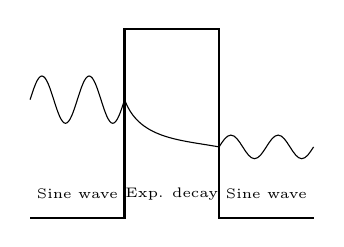
\begin{tikzpicture}[scale=0.6]
    % Border
    \draw[thick] (0,0) -- (2,0) -- (2,4) -- (4,4) -- (4,0) -- (6,0);
    
    % Sine waves
    \draw (0,2.5) sin (0.25,3.0) cos (0.5,2.5) sin (0.75,2.0) cos (1,2.5) sin (1.25,3.0) cos (1.5,2.5) sin (1.75,2.0) cos (2,2.5);
    \draw (2,2.5) to[out=290,in=170] (4,1.5);
    \draw (4,1.5) sin (4.25,1.75) cos (4.5,1.5) sin (4.75,1.25) cos (5,1.5) sin (5.25,1.75) cos (5.5,1.5) sin (5.75,1.25) cos (6,1.5);
    
    % Text
    \node at (1,0.5) {\tiny Sine wave};
    \node at (3,0.5) {\tiny Exp. decay};
    \node at (5,0.5) {\tiny Sine wave};
    
\end{tikzpicture}
\end{figure}

The wave functions in the 3 regions are
\begin{align}
    \Psi_{I}(x) &= A_1 e^{ikx} + A_2 e^{-ikx} \\
    \Psi_{II}(x) &= B_1 e^{\alpha x} + B_2 e^{-\alpha x} \\
    \Psi_{III}(x) &= C_1 e^{ikx} + C_2 e^{-ikx} 
\end{align}
Applying the boundary conditions leads to a transmission coefficient
\begin{equation}
    T = \frac{\left| \Psi_{III}(x) \right|^2}{\left| \Psi_{I}(\text{incident}) \right|^2} = T_0 e^{-2\alpha a}
\end{equation}
with
\begin{equation}
    T_0 = 16 E(V_0-E)V_0^{-2}
\end{equation}

\subsection{Hydrogen Atom}
Schrödinger equation with potential
\begin{equation}
    V(r) = -\frac{Z e^2}{4 \pi \varepsilon_0 r}
\end{equation}
%TODO: draw prob density and energy states

\subsection{Pauli Exclusion Principle}
%TODO: add relevant stuff

\subsection{Helium Atom}
Potential energy of an electron in Helium
\begin{equation}
    V(r_1,r_{12}) = -\frac{2e^2}{4 \pi \varepsilon_0 r_1} + \frac{e^2}{4 \pi \varepsilon_0 r_{12}}
\end{equation}